\documentclass[manuscript,screen,review]{acmart}
\acmJournal{TECS}
\setcopyright{none}
\settopmatter{printacmref=false}
\usepackage{tikz}
\usepackage{pgfplots}
\usepackage{placeins}
\pgfplotsset{compat=1.18}
\graphicspath{{figures/}}
\newcommand{\faultset}{A}
\newcommand{\protset}{P}
\newcommand{\risk}{R}
\newcommand{\E}{\mathbb{E}}
\newcommand{\Prob}{\mathbb{P}}
\newcommand{\bits}{\mathcal B}
\newcommand{\evidence}[1]{\textsf{#1}}
\newcommand{\CE}{\mathrm{CE}}
\newcommand{\AUC}{\mathrm{AUC}}

\title[Conditional Fault Vulnerability in Quantized Networks]{Beyond Isolated Bit Sensitivity: Conditional Fault Vulnerability and Protection-Allocation Limits in Quantized Neural Networks}
\author{Manuel Blanco Valentin}
\affiliation{\institution{Northwestern University}\city{Evanston}\state{Illinois}\country{USA}}
\renewcommand{\shortauthors}{Blanco Valentin}
\keywords{quantized neural networks, encoded-bit faults, conditional vulnerability, selective protection, interaction attribution, reproducible evaluation}

\begin{document}
\begin{abstract}
Selective protection of quantized neural networks often assigns a fixed score to each stored parameter bit. We investigate when isolated encoded-bit sensitivity is informative about protection value under simultaneous independent Bernoulli faults. We formulate exact task risk on fault sets and connect protection benefit to conditional probability-space derivatives, using established multilinear and Boolean-function foundations. An exact response-table decomposition separates clean isolated effects, outside-background conditioning, and interactions among candidate bits. Experiments use frozen INT8 TensorFlow Lite reference execution on keyword spotting, ResNet-8 image classification, and ToyCar anomaly detection, with complete-file ROC-AUC for the latter. An exploratory frozen-mask replication resolves a small conditional-selection benefit, but the selected-versus-exact-isolated intervals span zero in all six subsequent cross-pool campaign/BER arms. Across their 56 pool/BER conditions, outside-conditioned additive predictions reverse far fewer mask orderings than clean isolated predictions; this is selection-data attribution, not proof of held-out optimizer superiority. We also audit gradient proxies and two distinct FKeras scoring forms, identifying budgets at which strict bit-tier rankings yield identical masks. A sharp bounded-risk remainder inequality and finite-field regret bound characterize an outside-conditioned singleton approximation, while bounded numerical checks expose both its usefulness and its limitations. The contribution is a reproducible account of context dependence, approximation error, decision uncertainty, and computational cost, not a universal protection optimizer or a physical mitigation implementation.
\end{abstract}
\maketitle
\section{Introduction}\label{sec:introduction}
Protecting every stored neural-network parameter can be more expensive than protecting a selected subset. Vulnerability ranking therefore has a practical role in embedded-system design: it identifies locations whose protection might preserve application behavior under a limited budget. Yet an inexpensive ranking typically measures a different object from the protection decision. The numerical jump of an encoded bit, a gradient-derived score, an exact isolated fault, and the value of suppressing that fault in an already corrupted model are not interchangeable.

This paper studies that distinction with frozen quantized executables. Let $R(A)$ denote the task risk after exactly the stored bits in $A$ have been XOR-flipped. The isolated effect is $R(\{b\})-R(\varnothing)$. Under simultaneous faults, the relevant difference instead involves $R(G\cup\{b\})-R(G)$ for a random background $G$. Both the fault process and the currently protected coordinates determine the distribution of $G$. Even an exact isolated-bit ranking can therefore choose a different protection mask from a context-dependent analysis. This statement follows from elementary counterexamples; whether the discrepancy matters in a real network is an empirical question.

Prior sensitivity-guided fault injection, selective protection, and learning-based allocation already recognize that bits differ in importance and that simple significance rules have exceptions~\cite{weng2024fkeras,weng2026priorifi,catalan2025redundancy,alobaidi2026selectiveeccdataset}. We do not claim to originate that observation, Boolean influence, or adaptive protection. Our focus is narrower: make the exact encoded-bit decision object explicit; separate different sources of interaction-driven prediction error; and measure whether improved conditional description translates into a statistically resolved protection benefit against a strong exact-isolated comparator.

\paragraph{Research questions.}
\textbf{RQ1:} How do structural, gradient, and Hessian-based static rankings relate to exact finite-bit effects and actual protected masks? \textbf{RQ2:} How much does an outside fault background change isolated effects and equal-budget mask orderings? \textbf{RQ3:} Does a restricted empirical selector improve independently evaluated risk over a frozen static allocation and an exact-isolated allocation? \textbf{RQ4:} When does a cheaper outside-conditioned singleton approximation reproduce the exact bounded-candidate decision, and what can be certified about its error?

\paragraph{Contributions.}
First, we specialize established multilinear-risk identities to exact quantized execution, including protection and equal-budget swap identities, nonmonotone counterexamples, and the distinction between weight derivatives and fault-probability derivatives. Second, we provide an exact decomposition of equal-budget contrasts into clean isolated, outside-background, and within-candidate components, with no truncation of candidate interactions in the reference calculation. Third, we report all recorded pools from six campaign/BER arms on three frozen model families, including complete-file anomaly-detection risk. Fourth, we give a bounded-risk remainder and finite-field regret analysis, tested against saved exact tables and separately labeled engineering checks.

The results constrain the narrative as much as they support it. A replication of one historically chosen eight-bit pool finds a small favorable held-out contrast. Subsequent probability-sampled six-bit pools do not resolve selected-versus-exact-isolated superiority in any campaign arm. Outside conditioning explains most observed selection-order changes, but those changes are not themselves a demonstration of better final decisions. This distinction is central to the contribution, not a caveat deferred to future work.

All measured protection is \emph{ideal logical event suppression} on stored INT8 kernels. We neither rank physical storage exposure nor claim measured ECC/TMR, ASIC area, power, timing, radiation reliability, or an optimal whole-network allocation. Sections~\ref{sec:related}--\ref{sec:allocation} establish the objects and methods; Sections~\ref{sec:experiments}--\ref{sec:results} describe the evidence and results; Section~\ref{sec:discussion} assesses their limits. Appendix~\ref{app:math} supplies proofs and the explicitly nonempirical spectral interpretation.

\section{Related Work and Scope}\label{sec:related}
\subsection{Sensitivity-guided fault injection}
FKeras ranks edge-network parameters using gradients and leading weight-Hessian eigenpairs and orders bits by significance tiers~\cite{weng2024fkeras}. Our audit distinguishes its printed score from the effective sum strategy in the pinned public implementation. We preserve both definitions, adapt them to a continuous companion of the frozen KWS model, and keep the original tier-first ordering. This is source-level and numerical correspondence, not reproduction of the paper's original hardware or datasets.

PrioriFI uses Hessian-based initialization and observed fault outcomes to prioritize subsequent injections~\cite{weng2026priorifi}. Finding sensitive locations efficiently differs from minimizing expected risk of a fixed protected set under an exogenous fault law. Nevertheless, this is direct prior art on feedback-guided fault analysis and exceptions to significance monotonicity. Neither multiple-fault evaluation nor adaptive use of previous outcomes is novel here. We make no efficiency comparison against an unexecuted PrioriFI implementation.

\subsection{Protection mechanisms and learned allocations}
Catal\'an \emph{et al.} investigate fixed and variable bit protection using redundancy in stored numerical representations~\cite{catalan2025redundancy}. Those mechanisms and their hardware costs differ from forcing selected fault coordinates clean. COLA studies correlated feature errors and combines error coding with architectural/training changes~\cite{yu2023cola}. Its error-correlation object is not the anchored finite-bit interaction of a fixed executable.

The public \emph{Learned or Ranked?} companion release~\cite{alobaidi2026selectiveeccdataset} is particularly relevant. It provides learned and rule-based policies, cost-matched held-out comparisons, BER sweeps, and layer-interaction diagnostics. The source snapshot includes layer/subset additivity and contextual marginal analyses. This rules out a broad claim that protection dependence or layer interactions have not been studied. Its layer-wise choices, word-level ECC variants, burst/interleaving laws, and accuracy--cost reward differ from our fixed-cardinality encoded-bit problem. We do not assert that its layer interactions equal our candidate-bit M\"obius coefficients, or that ideal suppression beats ECC. The release is a dataset; peer-reviewed publication of the accompanying manuscript has not been established in our audit.

\subsection{Established mathematical foundations}
Multilinear extensions and biased Fourier analysis of functions on the Boolean cube are established tools~\cite{odonnell2014analysis}. Classical reliability importance also uses the difference between forced component states averaged over the remaining system~\cite{rauzy2022reliability}. Our signed, real-valued task risk need not be monotone, unlike a coherent failure indicator. Applying these identities to encoded neural-network faults does not make the identities new. Our claimed contribution is their operational separation and controlled validation on exact executables, including selection versus independent evaluation, nonadditive task metrics, and explicit approximation limits.

The resulting comparison is deliberately not a claim that static methods have no interactions and conditional methods do. A continuous Hessian contains cross-parameter curvature. A finite single-bit jump can be large; a projected parameter score need not estimate a probability-space derivative conditioned on protection. Conversely, an exact conditional measurement on a small candidate pool does not establish a globally optimal protection policy. These distinctions determine the baselines and claim boundaries throughout the paper.

\section{Exact Encoded-Bit Fault Model}\label{sec:fault}
\subsection{Storage and executable identity}
The eligible population $\bits=\{1,\ldots,N\}$ consists of allocated INT8 kernel bits. A bit identity contains the TFLite tensor, C-order word index, and bit position $j\in\{0,\ldots,7\}$. Kernels include depthwise and pointwise convolutions where present. INT32 biases, activation buffers, quantization metadata, code, and control state are excluded. A stored zero remains eligible; it is not a physically removed connection.

For affine decoding $w=s(q-z)$, let $a_j$ be bit $j$ of the two's-complement code. Its exact numerical displacement is
\begin{equation}\label{eq:xor-delta}
\delta_b=\begin{cases}s(1-2a_j)2^j,&j<7,\\-s(1-2a_7)2^7,&j=7.\end{cases}
\end{equation}
The scale $s$ follows the actual per-tensor or per-channel metadata; the zero point cancels in this difference. Faults XOR the stored codes used by authoritative inference, not floating-point shadow weights. Several distinct bits in one word compose by XOR, including sign changes. Exact baseline bytes are restored after each evaluated fault state.

\subsection{Risk and evaluation unit}
For a fixed input cohort $\mathcal D$, $R_{\mathcal D}(A)$ is the scalar risk of the executable with exactly $A$ flipped; we omit $\mathcal D$ when fixed. Classification risk is mean categorical cross-entropy from decoded integer-softmax probabilities, with true-class probability floored at $10^{-12}$, in nats per input. Accuracy is a separate descriptive endpoint. The clipping bounds this recorded risk by $L=-\log(10^{-12})$, not the unbounded cross-entropy of arbitrary continuous logits.

ToyCar risk is $1-\AUC$ on complete files. Let $s_f(A)$ be the pinned score obtained by aggregating all reconstruction windows of file $f$, and let $\mathcal F_+,\mathcal F_-$ denote anomalous and normal files. Then
\begin{equation}\label{eq:auc}
\AUC(A)=\frac{1}{|\mathcal F_+||\mathcal F_-|}\sum_{u\in\mathcal F_+}\sum_{v\in\mathcal F_-}
\left[\mathbf1\{s_u(A)>s_v(A)\}+\tfrac12\mathbf1\{s_u(A)=s_v(A)\}\right].
\end{equation}
One fault configuration persists across every window and file in the cohort. AUC is neither a window loss nor an average of per-file AUCs. Comparing normal/anomalous pairs does not make those pairs independent observations. ToyCar has $0\le R\le1$.

\subsection{Fault law and protection}
Let $Z\subseteq\bits$ include each bit independently with probability $p$. The fault field is persistent for one whole evaluation trial, then replaced independently. A fixed protected set $P$ applies ideal event suppression: only $Z\setminus P$ is executed. Thus
\begin{equation}\label{eq:expected-risk}
J_p(P)=\E_Z R(Z\setminus P).
\end{equation}
The budget in our comparisons is an \emph{exact cardinality} $|P|=B$. For nonmonotone risk, this is different from an at-most-$B$ budget: suppressing a beneficial fault can increase risk. No negative effect is clipped away.

All policies at a condition share proposed fields; proposed events equal applied plus suppressed events. With $B$ protected bits, the expectations are $Np$ proposed and $(N-B)p$ applied flips. Equal BER therefore does not match fault multiplicity across different model sizes. This law is a logical stress model, not a calibrated SEU rate, storage-occupancy model, or radiation cross section. Correlated/fixed-count faults and physical ECC decoding do not automatically obey the same protection coupling.

\section{From Isolated Sensitivity to Conditional Vulnerability}\label{sec:susceptibility}
\subsection{Fault-set and probability-space objects}
The exact isolated effect is $I_b=R(\{b\})-R(\varnothing)$. Define anchored coefficients
\begin{equation}\label{eq:mobius}
I_S=\sum_{T\subseteq S}(-1)^{|S|-|T|}R(T),\qquad R(A)=\sum_{S\subseteq A}I_S.
\end{equation}
In particular $I_{bc}=R(\{b,c\})-R(\{b\})-R(\{c\})+R(\varnothing)$. These are finite differences of exact executable risk, not a Taylor expansion.

For independent coordinate probabilities $\mathbf q$, the multilinear extension is
\begin{equation}\label{eq:multi-extension}
F(\mathbf q)=\E_{Z\sim\mathbf q}R(Z)=\sum_{S\subseteq\bits}I_S\prod_{b\in S}q_b.
\end{equation}
Conditioning on coordinate $b$ gives
\begin{equation}\label{eq:prob-gradient}
V_b(\mathbf q_{-b})=\partial_b F(\mathbf q)=\E_G[R(G\cup\{b\})-R(G)],
\end{equation}
where $G$ excludes $b$ and follows the other coordinate probabilities. This first probability derivative contains every interaction order involving $b$: $I_b+\sum_{c\ne b}q_cI_{bc}+\cdots$. For $b\ne c$, $\partial_{bc}F$ is the corresponding background-averaged four-state finite difference; $\partial_{bb}F=0$. No differentiability of integer inference is assumed. These identities follow from established multilinear theory, not a new neural-network calculus~\cite{odonnell2014analysis,rauzy2022reliability}.

Set $q_b=0$ on $P$ and $p$ otherwise. For $b\notin P$, multi-affinity gives the exact benefit
\begin{equation}\label{eq:protection-benefit}
J_p(P)-J_p(P\cup\{b\})=p V_b(p,P).
\end{equation}
Thus isolated damage is the zero-background limit, not the general finite-BER protection value. $V_b$ is signed; it is not the absolute Boolean influence sometimes used to measure sensitivity without direction.

\subsection{Static estimators and their distinct objectives}\label{sec:estimators}
For the companion's per-input loss $\ell_x$, write $z_b(x)=\partial\ell_x/\partial w_b\,\delta_b$. Our static definitions are:
\begin{align}
S2_b&=j_b \quad\text{(descending word-relative significance)},\nonumber\\
S3_b&=|\delta_b|,\qquad
S4_b=|\E_x z_b(x)|,\label{eq:static}\\
S5_b&=\E_x|z_b(x)|,\qquad
S6_b=\E_x\max(0,z_b(x)).\nonumber
\end{align}
S4 saves the signed prediction $\E z$ separately but ranks its magnitude. S5 targets absolute per-input sensitivity; S6 targets positive first-order per-input changes. Neither is an exact prediction of positive aggregate risk damage. Random uses a recorded seed. All methods use the same eligible population and deterministic tie rules; estimator score, ordering policy, mask selection, and mitigation remain separate.

For $S5_b>0$, directional coherence $C_b=\E z_b/S5_b$ satisfies $S6_b=S5_b(1+C_b)/2$. This is an algebraic identity when the same contributions are aggregated. Separate float32 reductions can differ numerically; it is not sound to infer coherence from incompatible transformed scores. Task alignment also matters: KWS/ResNet companions use a classification loss, while ToyCar gradients use reconstruction MSE, not differentiable AUC.

The companions preserve kernel-variable identities and exact affine bit jumps but use straight-through activation requantization. Their derivatives are hypotheses about exact integer faults, not derivatives of the discrete program. Forward discrepancies, saturation, large sign-bit perturbations, and changed fault context can invalidate local approximations. Exact isolated effects and protection outcomes always use the authoritative backend.

\subsection{Faithful scope of the FKeras baseline}
The printed FKeras parameter vector is $h=\sum_{i=1}^k\lambda_i(v_i^\top\theta)v_i$~\cite{weng2024fkeras}. We record that signed vector and use $|h|$ within significance tiers. The pinned repository's \texttt{sum} strategy instead gives $\sum_i|\lambda_i^2(v_i^\top\theta)v_i|$~\cite{fkerasSource}. Multiplying the vector by its eigenvalue before both the dot product and final product introduces the square; componentwise magnitudes precede summation. With one nonzero eigenpair the magnitude rankings are proportional, but multiple eigenpairs can change weighting and cancellation. Both variants are reported; neither is selected for favorable outcomes.

For KWS we use a separately identified float64 continuous companion with decoded kernels, fixed decoded biases, and no activation requantization. Deterministic symmetric Lanczos targets signed eigenvalues of largest magnitude, retaining negative values. Orthogonality, symmetry, normalized residuals, dense small-network references, and finite-difference Hessian-vector products are checked. This reproduces the scoring forms on validated eigenpairs, not the upstream eigensolver's every numerical behavior or the original QKeras experiments. It is also a different surrogate from S4--S6.

FKeras remains tier-first, with sensitivity only within a tier. For homogeneous INT8 storage, 12.5\% protection selects every sign bit and 25\% selects every sign and bit-6 position. These masks must equal corrected MSB-first regardless of parameter sensitivity. Partial-tier budgets can distinguish them. A continuous weight Hessian can contain cross-parameter interactions, but this projected score does not condition on the current protection mask or Bernoulli background. We do not characterize it as a diagonal Hessian or as a full conditional oracle.

\section{Exact Restricted Decisions and Approximation Limits}\label{sec:allocation}
\subsection{A complete counterexample}
Consider $R(z_1,z_2,z_3)=1.2z_1+z_2+0.1z_3+3z_2z_3$. Exact isolated damage ranks $1>2>3$. With one protected bit,
\begin{equation}\label{eq:counterexample}
J_p(\{1\})=1.1p+3p^2,\quad J_p(\{2\})=1.3p,\quad J_p(\{3\})=2.2p.
\end{equation}
The optimal choice switches from bit 1 to bit 2 at $p=1/15$. There is no estimation error. This disproves universal isolated-ranking optimality, not the usefulness of static rankings on a particular network.
\begin{figure}[t]
\centering
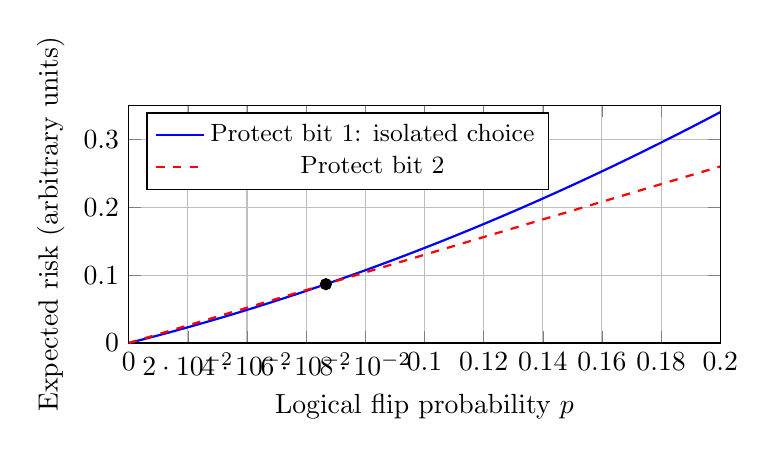
\begin{tikzpicture}
\begin{axis}[width=.75\linewidth,height=4.6cm,xlabel={Logical flip probability $p$},ylabel={Expected risk (arbitrary units)},xmin=0,xmax=.2,ymin=0,ymax=.35,grid=major,legend pos=north west,domain=0:.2,samples=101,legend style={font=\small}]
\addplot[thick,blue] {1.1*x+3*x^2};\addlegendentry{Protect bit 1: isolated choice}
\addplot[thick,red,dashed] {1.3*x};\addlegendentry{Protect bit 2}
\addplot[only marks,black] coordinates {(.0666666667,.0866666667)};
\end{axis}
\end{tikzpicture}
\caption{Analytical counterexample, not a measured neural-network result. The exact isolated ranking is optimal only below the crossing.}\label{fig:counterexample}
\Description{Two analytical risk curves cross at logical flip probability one fifteenth.}
\end{figure}

\subsection{Fixed global context and response-table reuse}
Let $P_0$ be a verified static mask, $C$ a frozen candidate pool of size $K$, and $r=|P_0\cap C|$. Fix $P_{\rm out}=P_0\setminus C$ and compare $P(Q)=P_{\rm out}\cup Q$ for every $Q\subseteq C$ with $|Q|=r$. The whole-network cardinality is unchanged. Draw $G$ only on coordinates outside $C\cup P_{\rm out}$ and evaluate $h_G(A)=R(G\cup A)$ for all $2^K$ candidate states. For $U=C\setminus Q$,
\begin{equation}\label{eq:exact-table}
J_G(Q)=\sum_{A\subseteq U}p^{|A|}(1-p)^{|U|-|A|}h_G(A),\qquad J_p(P(Q))=\E_G J_G(Q).
\end{equation}
One response table supports all eligible masks without further inference and retains every candidate interaction order. Exact candidate integration removes candidate-draw Monte Carlo noise, not outside-field or input-cohort uncertainty. The conditional equivalence between forcing a bit clean and suppressing it relies on the independent product law; it need not hold under correlated or fixed-count faults.

Masks are selected on model-selection cohorts and outside fields only. The original static mask, the exact-isolated comparator (largest signed clean single-bit effects on the selection cohort), and the minimum empirical integrated-risk mask are frozen before final evaluation. Exactness refers to executable effects and candidate integration; the selected mask minimizes a \emph{finite-field restricted} objective, not whole-network expected risk.

For a swap releasing $a\in P$ and protecting $b\notin P$, let $P'=(P\setminus\{a\})\cup\{b\}$. With the same Bernoulli background over coordinates unprotected under both masks,
\begin{equation}\label{eq:swap}
J_p(P')-J_p(P)=p\,\E_G[R(G\cup\{a\})-R(G\cup\{b\})].
\end{equation}
Final comparisons use this paired-swap identity along fixed paths; all path steps are summed within a master field before uncertainty is calculated. It remains valid for scalar cohort AUC. It does not assume an additive per-input risk or implement a new optimizer.

\subsection{An exact attribution of decision differences}\label{sec:decomposition}
On the \emph{same} selection cohort define $R_0=R(\varnothing)$, $d_b^0=R(\{b\})-R_0$, and $d_b^G=h_G(\{b\})-h_G(\varnothing)$. Then
\begin{align}\label{eq:decomposition}
J_G(Q)={}&\underbrace{R_0+p\sum_{b\in U}d_b^0}_{\text{clean isolated prediction}}
+\underbrace{h_G(\varnothing)-R_0}_{\text{background intercept}}\nonumber\\
&+\underbrace{p\sum_{b\in U}(d_b^G-d_b^0)}_{\text{outside-background correction}}
+\underbrace{J_G(Q)-h_G(\varnothing)-p\sum_{b\in U}d_b^G}_{\text{within-candidate correction}}.
\end{align}
The intercept cancels between masks. The remaining signed terms close exactly for every equal-budget contrast. Averaging absolute terms and signed terms answers different questions; cancellation can hide heterogeneous field effects. This is algebraic attribution, not proof that neural redundancy or gating caused an architectural difference.

Importantly, $d_b^G$ forces \emph{all other candidates clean}. Its outside-field mean is not the full $V_b$ in Eq.~\eqref{eq:prob-gradient}, which also averages unprotected candidate faults. For $h(A)=\mathbf1\{\{1,2,3\}\subseteq A\}$, every singleton response is zero but the full conditional vulnerability is $p^2$. A $K+1$-state approximation cannot be renamed an exact conditional oracle.

\subsection{Bounded-risk error and restricted regret}\label{sec:bounds}
Write $A_p(Q)=\E h_G(\varnothing)+p\sum_{b\in U}\E d_b^G$, and $E_{\ge2}(Q)=J_p(P(Q))-A_p(Q)$. If $0\le R\le L$ and $m=K-r\ge2$, then
\begin{equation}\label{eq:bound}
|E_{\ge2}(Q)|\le\epsilon_m=Lmp[1-(1-p)^{m-1}].
\end{equation}
The remainder is zero for $m\le1$. The bound is sharp without monotonicity assumptions: $h(\varnothing)=L$, singleton risks zero, and all multi-fault risks $L$ attain it. In particular, replacing the right side by $L\Prob(|A|\ge2)$ is invalid; the singleton linearization can overshoot the risk range. The proof is in Appendix~\ref{app:math}.

If $Q_A$ minimizes the outside-additive function and $Q_*$ minimizes exact expected risk in the same restricted family, the regret is at most $\min(L,2\epsilon_m)$. For $n$ independent outside fields, define $t=L\sqrt{2\log(2K/\alpha)/n}$. Hoeffding's inequality and an equal-budget cancellation argument give, with probability at least $1-\alpha$,
\begin{equation}\label{eq:samplebound}
J_p(P(\widehat Q_A))-J_p(P(Q_*))
\le \min\{L,2\epsilon_m+2p\min(r,K-r)t\}.
\end{equation}
This conditions on a frozen pool, model and cohort. Shared fields across bits are allowed; independent fields across observations are required. The approximation bias and field-estimation uncertainty are separate.

A globally certified bound $\kappa_{bc}$ on every contextual second difference yields the alternative $p^2\sum_{b<c\in U}\kappa_{bc}$. Maxima over recorded fields certify only those recorded fields. Empty-context pair differences alone cannot bound pure third-order effects. The inequalities clarify limits, but a numerically loose certificate is not evidence that a small observed decision difference is practically resolved.

\section{Experimental Protocol}\label{sec:experiments}
\subsection{Frozen models and exact execution}
Table~\ref{tab:models} identifies the three kernel-only populations. The models and preprocessing descend from pinned MLPerf Tiny assets~\cite{banbury2021mlperf,mlcommons2026tiny}, not newly trained checkpoints. Authoritative inference is TensorFlow Lite 2.14.1, \texttt{BUILTIN\_REF}, one inference thread, no delegates. Locks bind model bytes, dataset identities, ordered inputs, scales, zero points, and clean-reference digests. Optimized kernels are not silently substituted. ToyCar preprocessing additionally preserves the validated two-thread BLAS reduction contract; this is separate from single-threaded TFLite execution.
\begin{table}[t]
\caption{Frozen model populations and task risk. Hash prefixes identify full SHA-256 values in the evidence manifest. All other state is nonfaultable.}\label{tab:models}
\centering\small
\begin{tabular}{lrrll}\toprule
Model & INT8 kernel words & Eligible bits & Risk & Model SHA prefix\\\midrule
DS-CNN KWS &22,016&176,128&CE&\texttt{aeea43680070}\\
ResNet-8 &77,360&618,880&CE&\texttt{3c002613d1b2}\\
ToyCar AD &264,192&2,113,536&$1-\AUC$&\texttt{87cf24194ef9}\\\bottomrule
\end{tabular}
\end{table}

KWS uses the pinned Speech Commands TFDS ordering, round-robin blocks of 16, waveform normalization, and the official MFCC pipeline. CIFAR-10 inputs preserve frozen indices and quantized preprocessing. ToyCar uses the official mel-power pipeline, five-frame concatenation and 196 reconstruction windows per selected complete file. Its score is the pinned mean reconstruction error against the float-domain target, not a newly normalized loss. Gradients use normal training data; labeled final cohorts do not train a ranking surrogate.

\subsection{Study lineage and partitions}
We use stable study identifiers to bind manuscript claims to finalized artifacts, not as independent statistical replications. \evidence{M9.5.2} evaluates ten explicitly chosen KWS bits on 256 training clips and 512 test clips, with 64 and 128 independent backgrounds respectively at each BER. The pool is descriptive, not a uniform sample. \evidence{M9.5.7} fixes an exploratory eight-bit pool and previously selected masks, then evaluates 256 new master fields on 256 clips (original test indices 3194--3449). Earlier conditional outcomes influenced the pool lineage; independent final fields do not erase that selection history.

The later campaigns sample six-bit pools, with two bits uniformly drawn from the source S5-protected population and four from its complement. Each pool has exactly two protected positions and 15 legal masks. This is a probability-sampled \emph{status-stratified pool design}, not six uniform whole-network bits. Source S5 protects 12.5\% of all eligible kernel bits, and $P_{\rm out}$ is held fixed while two positions are exchanged. All planned pools are retained, including identical-mask and adverse cases.
\begin{table}[t]
\caption{Completed restricted campaigns. Selection and final counts are independent outside/master fields per pool. Inputs are fixed within an arm. A and B denote different KWS cohort windows, not different checkpoints.}\label{tab:design}
\centering\small
\begin{tabular}{llrrrrl}\toprule
Evidence & Model/arm & $p$ & Pools & Fields sel./final & Inputs sel./final & Risk\\\midrule
M9.6 &KWS A&.01&12&32/128&64/512 clips&CE\\
M9.7 &KWS B&.001&12&32/128&64/512 clips&CE\\
M9.7 &KWS B&.003&12&32/128&64/512 clips&CE\\
M9.7 &KWS B&.01&12&32/128&64/512 clips&CE\\
M9.8 &ResNet-8&.01&4&8/32&32/128 images&CE\\
M9.9 &ToyCar&.001&4&8/32&24/48 files&$1-\AUC$\\\bottomrule
\end{tabular}
\end{table}

KWS A selection/final indices are 2088--2151/3450--3961; KWS B uses 2152--2215/3962--4473. The same twelve candidate pools recur across these arms, so 48 KWS pool/BER records are not 48 independently sampled pools. ResNet uses 1024--1055/3225--3352. ToyCar selection comprises normal files 64--75 and anomalous files 204--215; final uses normal 76--99 and anomalous 216--239. These are source indices, with exact file IDs and order in manifests. Disjoint source windows do not establish identical class or device distributions.

The frozen protocol separates calibration, selection-only execution, sealed masks, and final-only comparisons. Exposure ledgers reject known reused confirmation windows. The ToyCar retrospective ledger records fault-outcome exposure for 200 of 248 official files and clean inference on all files; only 40 normal and eight anomalous files remain without recorded fault outcomes. Its completed study is consequently exploratory evidence on an already extensively examined dataset, not external confirmation. Undocumented manual or failed jobs cannot be excluded by a finalized-bundle ledger.

\subsection{Statistics and decision units}
Whole fault fields are independent Monte Carlo units conditional on model, masks, and inputs. Paths, candidate pairs, and policies sharing a field are not independent trials. Final comparisons are target-minus-baseline risk; negative favors the target. Pool-level summaries equally weight pool means, with marginal Student-$t$ intervals using pools as units. These intervals are descriptive conditional approximations, particularly with four pools, not input-population guarantees or robust proofs under unseen heavy tails.

The original protocols preserve different comparison families. M9.5.7 has one primary selected-minus-S5 comparison and two Holm-adjusted secondary comparisons. M9.6/M9.8/M9.9 similarly distinguish the primary comparison from two secondary pool-level contrasts. The M9.7 joint protocol has two primary across-BER contrast changes and a nine-test within-BER secondary family, with Holm adjustment and separately saved simultaneous intervals. The marginal intervals shown here do not replace those families, and their overlap is not a significance test. New M9.10 attribution and input-resampling analyses are explicitly exploratory. Stratified complete-file resampling recomputes ToyCar AUC; neither windows nor normal/anomalous pairs are resampled as independent files.

Static empirical validation uses 320 bits: four per tensor-by-bit-position stratum across ten kernels. Recorded inclusion probabilities differ by tensor size. Correlations and top-$k$ recall describe this balanced sampled set, not an unbiased whole-network top-$k$ population. Fixed-mask fault replications are distinct from independent random-mask seeds. The later exact response-table analysis does not change any earlier estimator, mask, cohort, seed, or raw measurement.

\subsection{Integrity and analysis provenance}
The publication package records full paths, SHA-256 identities, source revisions, artifact selectors, and figure/table derivations. Source payloads and consumed artifacts are checked before use; large unused prediction tables are not claimed to have been rehashed in this manuscript pass. The M9.10 derivation originally verified complete source inventories and every exact response state; its finalized derived files and all 112 selection/final payload identities are independently checked again here. No model inference, mask generation, training, or scientific rerun was performed to author this draft. The M11 planned large-scale studies are not empirical evidence.

\section{Results: Context Dependence and Decision Limits}\label{sec:results}
\subsection{Static proxies: useful but not universal}
Table~\ref{tab:static-validation} reports the saved associations with positive isolated \emph{loss} damage. The gradients carry information on these balanced candidate sets, but the intervals are not pairwise tests of estimator superiority. ToyCar's target here is reconstruction MSE, not AUC. A useful MSE ranking need not protect anomaly-score ordering.
\begin{table}[t]
\caption{Sample-limited Spearman association on 320 stratified candidates per model. Intervals resample within recorded strata. Random is one saved seeded draw. Recorded runtime zeros for arithmetic/random baselines do not imply zero cost; S5/S6 share gradient computation and their rows must not be added.}\label{tab:static-validation}
\centering\small
\begin{tabular}{llrrr}\toprule
Model/loss&Score&$\rho$&Sample-design 95\% interval&Seconds\\\midrule
\csname @@input\endcsname tables/static_rank_validation.tex 
\bottomrule\end{tabular}
\end{table}

The static protection contrasts at BER .01 in Table~\ref{tab:static-protection} show why isolated predictive association is insufficient. S5 improves ResNet accuracy relative to corrected MSB in this recorded condition, whereas KWS effects are much smaller and ToyCar results depend on budget. These are task-specific effects, not evidence of a common architectural mechanism. Both interior budgets are retained rather than choosing the favorable one. All BERs and paired comparisons remain in the evidence supplement.
\begin{table}[t]
\caption{Saved paired S5-minus-MSB task-metric effects at logical BER .01. Positive favors S5. ResNet/KWS values are accuracy fractions; ToyCar values are AUC differences. Holm values retain each source's within-BER/metric family. This retrospective table is not a new confirmatory family.}\label{tab:static-protection}
\centering\small
\begin{tabular}{lrrrrr}\toprule
Model&Coverage&Fields&Effect&95\% paired interval&Holm $p$\\\midrule
\csname @@input\endcsname tables/static_comparison.tex 
\bottomrule\end{tabular}
\end{table}

\subsection{FKeras: verified numerical distinctions, limited efficacy evidence}
The KWS engineering eigensolve uses two calibration clips and two eigenpairs. Eigenvalues are approximately 5341.9031 and 434.7146, with normalized residuals $3.27\times10^{-16}$ and $3.04\times10^{-12}$, orthogonality error $6.87\times10^{-16}$, and 25 Hessian-vector products. These validate the continuous calculation, not Taylor accuracy for large encoded faults. Finite-difference checks pass in sufficiently small ReLU-stable neighborhoods; coarser steps crossing gates do not pass.

Actual masks differ between paper and repository forms at partial tiers (Table~\ref{tab:fkeras}), but coincide at complete tiers. The bounded matched protection check uses two fields and four test clips; every method retains accuracy 1.0, while CE varies and beneficial perturbations are retained. It cannot establish Hessian ranking superiority. Saved construction times are approximately 0.354 seconds for S4, 3.562 shared seconds for S5/S6, and 1.125 shared seconds for the FKeras variants. The saved coordinator elapsed time is 61.48 seconds, including loading and orchestration outside the timed score calculations. These setup-dominated measurements are not scalable throughput claims.
\begin{table}[t]
\caption{Exact symmetric differences between full KWS protection masks in the FKeras engineering check. Paper/repository differ by 901 exchanged positions at partial tiers. Equal masks under paired fields must give equal results.}\label{tab:fkeras}
\centering\small
\begin{tabular}{rrrrr}\toprule
Coverage&Protected bits&Paper/repository&MSB/paper&MSB/repository\\\midrule
\csname @@input\endcsname tables/fkeras_masks.tex 
\bottomrule\end{tabular}
\end{table}

\subsection{Exact conditional effects and the exploratory frozen pool}
M9.5.2 directly changes the background while retaining each bit identity. At $p=0$, conditional and isolated effects agree. At positive BER, point orderings change in both sample partitions (Table~\ref{tab:conditional-ranks}). These reversals share candidates and fields and are not independent binomial trials. Figure~\ref{fig:conditional} shows all ten held-out candidates rather than only a sign-changing example.
\begin{table}[t]
\caption{M9.5.2 exact isolated versus estimated conditional ordering for ten explicit KWS bits. Train/test use 64/128 fields and 256/512 clips. Spearman concerns these ten bits only.}\label{tab:conditional-ranks}
\centering\small
\begin{tabular}{lrrr}\toprule
Split&BER&Strict reversals/comparable pairs&Spearman\\\midrule
\csname @@input\endcsname tables/conditional_ranks.tex 
\bottomrule\end{tabular}
\end{table}
\begin{figure}[t]
\centering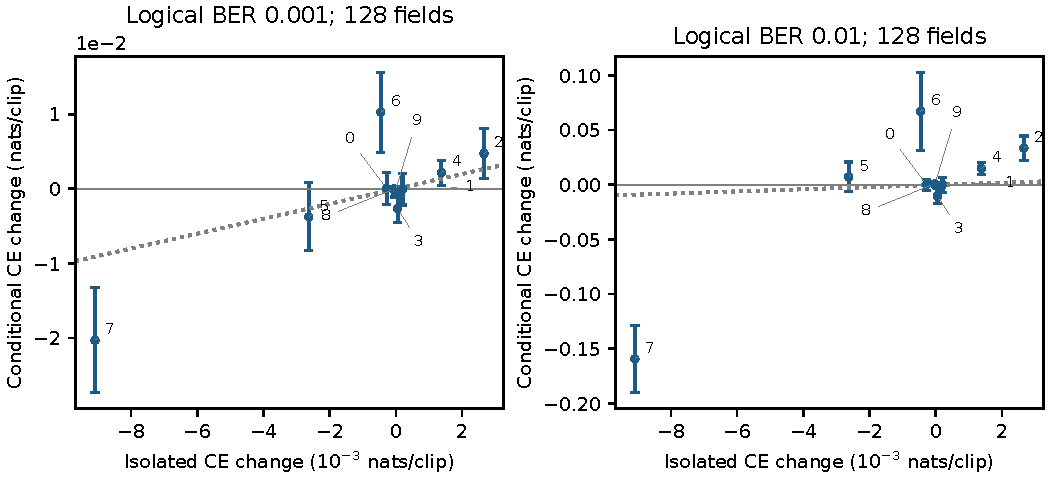
\includegraphics[width=\linewidth]{conditional_damage.pdf}
\caption{Exact isolated CE change versus mean conditional change, M9.5.2. Vertical bars are marginal field-level 95\% intervals conditional on the fixed 512 clips. Numbers index the same ten frozen candidates across panels. Beneficial and harmful changes remain signed; intervals are not adjusted for selecting a favorable bit.}\label{fig:conditional}
\Description{Two panels show all ten exact isolated effects and conditional means at BER .001 and .01 with error bars; the equality line does not describe many of the observations.}
\end{figure}

M9.5.7 independently evaluates previously frozen masks in one exploratory eight-bit pool. Selected, exact-isolated and original S5 masks protect local indices $(2,6)$, $(2,7)$ and $(6,7)$ respectively, with a global budget of 22,016 bits. Table~\ref{tab:replication} reports the positive evidence without treating the chosen pool as representative. The selected-versus-isolated secondary Holm value is $1.70\times10^{-28}$ under the saved paired-$t$ procedure. The mean CE benefit is small in absolute units. The selected-minus-S5 median is about $-1.80\times10^{-4}$, and eight of 256 fields are adverse; every field is retained. This result establishes a fixed-mask contrast under that protocol, not a population-wide ranking advantage.
\begin{table}[t]
\caption{M9.5.7 exploratory frozen-mask replication: 256 paired master fields, 256 fixed clips, BER .01. Negative CE favors the left method. Intervals are marginal field-level 95\% $t$ intervals, not pool-population intervals.}\label{tab:replication}
\centering\small
\begin{tabular}{lrrr}\toprule
Contrast&Mean CE difference&95\% interval&Favorable fields\\\midrule
\csname @@input\endcsname tables/frozen_replication.tex 
\bottomrule\end{tabular}
\end{table}

\subsection{All-pool independent evaluation does not resolve isolated-oracle superiority}
Table~\ref{tab:heldout} and Fig.~\ref{fig:heldout} retain all six completed campaign/BER arms. Selected-minus-S5 means are negative for all KWS arms. The more demanding selected-minus-exact-isolated marginal intervals span zero in \emph{every} arm. ResNet and ToyCar even have positive selected-minus-isolated means. These findings do not establish equality; they show that superiority is unresolved at the available sampling budgets.
\begin{table}[t]
\caption{Independent final target-minus-baseline risk for the restricted-selected mask. Equal-pool means and marginal 95\% pool-$t$ intervals; negative favors selected. CE and $1-\AUC$ retain separate units. All masks, including coincidences, remain included.}\label{tab:heldout}
\centering\small
\begin{tabular}{lllrll}\toprule
Campaign&BER&Baseline&Pools&Mean risk difference&95\% interval\\\midrule
\csname @@input\endcsname tables/heldout.tex 
\bottomrule\end{tabular}
\end{table}
\begin{figure}[t]
\centering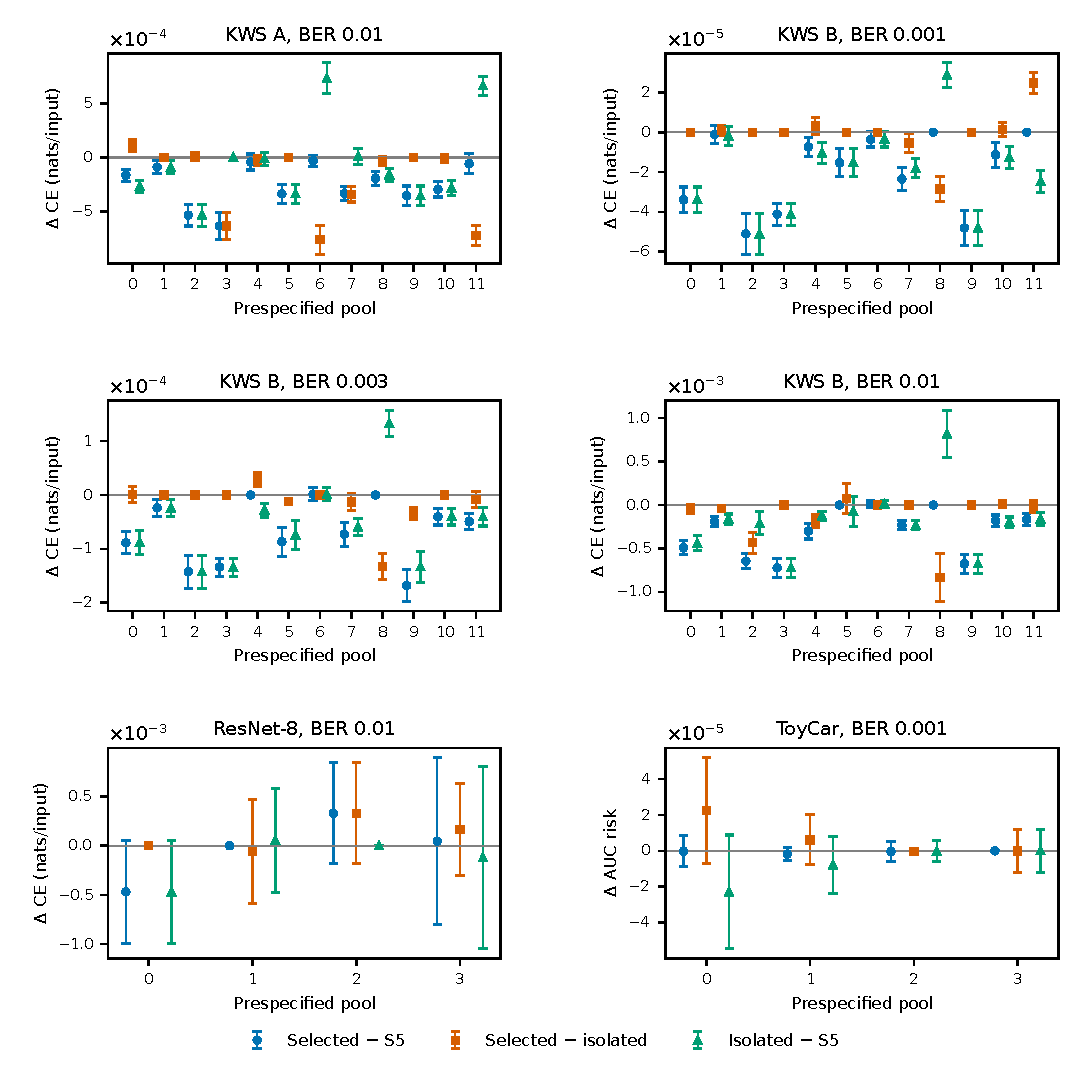
\includegraphics[width=\linewidth]{heldout_pool_effects_paper.pdf}
\caption{All finalized M9.10 held-out pool contrasts with saved marginal paired-field 95\% intervals; equal-pool intervals are in Table~\ref{tab:heldout}, not this plot. Panels retain distinct risk units and scales. The recurring twelve KWS pools do not create new independent pools at each BER.}\label{fig:heldout}
\Description{Six panels display all held-out paired mask effects and field-level intervals, including zero and adverse cases.}
\end{figure}

The exploratory eight-bit result and these six-bit campaigns answer different questions: the first fixes a historically informed pool; the latter sample pools within source-mask status strata. Different cohorts and field counts also intervene. Selecting favorable later pools to reproduce the earlier result would invalidate the generalization question. No such filtering is used.

\subsection{Outside conditioning dominates recorded selection reordering}
The exact signed decomposition closes to a maximum absolute residual of $3.55\times10^{-15}$ across recorded fields and masks. Clean isolated predictions produce many strict mask-order reversals, while background-conditioned singleton predictions produce few (Table~\ref{tab:reversals}). The latter can still miss nonzero interactions; decision contributions are weighted by $p^2,p^3,\ldots$ and need not reflect the size of forced multi-bit effects.
\begin{table}[t]
\caption{Selection-mask order reversals against exact candidate integration. Denominators count strict comparable pairs after a diagnostic $10^{-12}$ near-tie exclusion; pairs are not independent observations. No mask is changed by the diagnostic threshold.}\label{tab:reversals}
\centering\small
\begin{tabular}{llrr}\toprule
Campaign&BER&Clean isolated&Outside-conditioned\\\midrule
\csname @@input\endcsname tables/reversals.tex 
\bottomrule\end{tabular}
\end{table}
\begin{table}[t]
\caption{Signed selection-data selected-minus-isolated attribution, equally averaged over all pools. The first three columns sum to the last. CE units apply except ToyCar, which is $1-\AUC$. These are post-selection descriptive contrasts, not unbiased held-out gains.}\label{tab:attribution}
\centering\small
\begin{tabular}{llllll}\toprule
Campaign&BER&Clean&Outside&Within candidate&Exact\\\midrule
\csname @@input\endcsname tables/attribution.tex 
\bottomrule\end{tabular}
\end{table}

Crucially, these are model-selection tables. The final paired-swap archive lacks complete final subcubes and matching same-final-cohort clean-isolated controls. We therefore cannot attribute a final risk contrast to these three components, nor assign selection/final disagreement uniquely to interaction, input shift, or field noise.

\subsection{ToyCar: real interactions, coarse cohorts, unresolved decisions}
The clean selection and final AUCs are 0.826389 and 0.920139 on balanced 24- and 48-file cohorts. One untied pair reversal changes their AUC by $1/144$ and $1/576$; ties receive half credit. This is single-state metric resolution, not a floor on expected differences, which may be much smaller after multiplication by $p$ and averaging.

Across the four pools, 390, 296, 332 and 288 of 504 nonempty forced candidate-state responses change AUC relative to their field's empty candidate state. These states are not equiprobable Bernoulli outcomes. Mean outside-field risks are roughly .45, .39, .44 and .44, showing substantial degradation despite tiny mask contrasts. The selected and original masks coincide in one pool, yielding a structurally zero selected-minus-S5 contrast there; other pools contain nonzero field effects. Neither the unresolved aggregate result nor small expected corrections imply an absence of interactions.
\begin{figure}[t]
\centering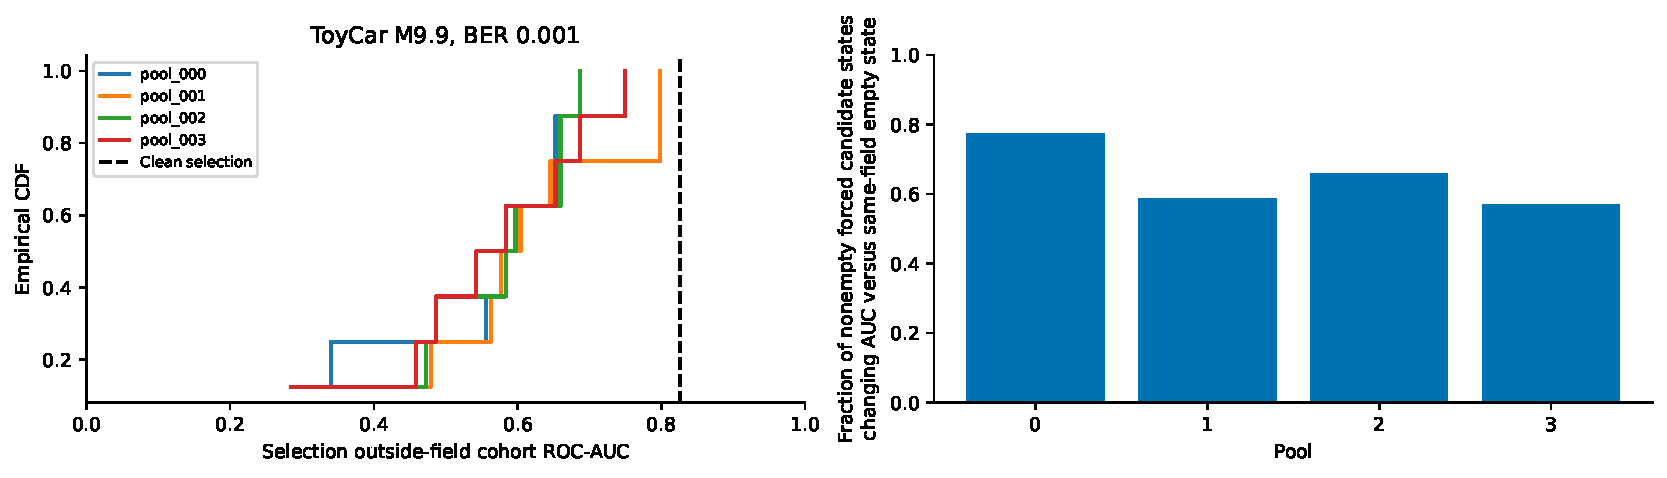
\includegraphics[width=\linewidth]{toycar_resolution.pdf}
\caption{Finalized complete-file ToyCar diagnostics: cohort metric resolution, background degradation and changes under forced candidate states. Forced states are diagnostics, not uniformly weighted deployment events. No window-wise AUC or additive file-loss substitution is made.}\label{fig:toycar}
\Description{ToyCar panels display clean and faulted cohort risks and how frequently forced candidate states change AUC, despite small expected protection contrasts.}
\end{figure}

\subsection{M11: approximation validation is not a large-scale efficacy result}
Reusing the 56 recorded exact pool/BER tables requires no new inference. Table~\ref{tab:approximation} shows that the outside-additive choice attains the recorded finite-field optimum in the classification arms, while ToyCar's mean finite-field regret is approximately $2.17\times10^{-10}$. This near-agreement is meaningful for these small low-occupancy candidate pools, not a certificate for larger pools, unseen fields or the final task population.
\begin{table}[t]
\caption{M11 offline reuse of all historical exact selection tables. Error is the pool-mean of maximum absolute mask-risk error; regrets compare choices on those same finite selection fields. These are not independent final performance estimates.}\label{tab:approximation}
\centering\small
\begin{tabular}{lllll}\toprule
Campaign&BER&Outside max error&Outside regret&Clean regret\\\midrule
\csname @@input\endcsname tables/approximation.tex 
\bottomrule\end{tabular}
\end{table}

Separate engineering checks use two previously exposed inputs (complete files for ToyCar), BER .003, and only one or two outside fields. KWS $K=8$ produces nonzero outside-additive regret, while $K=12$ has many strict ordering reversals but zero decision regret on the recorded field (Table~\ref{tab:oracle}). Ranking agreement and decision quality are therefore different objectives. Small ToyCar checks are especially coarse. No large-$K$ optimum or broad protection advantage was measured.
\begin{table}[t]
\caption{Bounded M11 outside-additive versus exact oracle checks, not publication efficacy trials. Times are recorded evaluation work including controls, excluding process startup. Each cohort has only two inputs/files.}\label{tab:oracle}
\centering\small
\begin{tabular}{lrrllrr}\toprule
Model&$K$&Fields&Max error&Selection regret&Reversals&Seconds\\\midrule
\csname @@input\endcsname tables/oracle.tex 
\bottomrule\end{tabular}
\end{table}

The formal bound is conservative here. For $K=6,r=2,p=.01$ and clipped classification CE, $\epsilon_m=0.03283$ nats, far larger than the recorded outside-additive errors and many final decision effects. ToyCar at $p=.001$ has $\epsilon_m\approx1.20\times10^{-5}$. Finite-field uncertainty increases the certificate further. The bound is useful for identifying assumptions and failure regimes; it does not statistically resolve the observed small differences.

\subsection{Computational cost}
Each $K=6$ selection field requires 64 cohort states and yields all 15 legal mask risks. The outside-singleton approximation needs seven states per field, but selecting well with it may still require many fields. At $K=8$ and 12 the corresponding reference/approximation counts are 256/9 and 4096/13. These are exact operation ratios, not measured end-to-end speedups.
\begin{table}[t]
\caption{Saved engine wall times summed across pools, in seconds. Setup is included. Concurrent campaign elapsed time and machine-independent throughput cannot be inferred from these sums.}\label{tab:costs}
\centering\small
\begin{tabular}{llrr}\toprule
Campaign&BER&Selection&Final\\\midrule
\csname @@input\endcsname tables/costs.tex 
\bottomrule\end{tabular}
\end{table}
A ToyCar cohort state evaluates every window of every complete file: 24 selection files imply 4,704 window inferences per state. The finalized M9.10 replay uses saved responses with no model calls. Costs and decision magnitudes must be considered together; response-table reuse saves new inference but cannot create information about unobserved final states.
\FloatBarrier

\section{Discussion and Threats to Validity}\label{sec:discussion}
\subsection{What is established}
Independent fault events can have interacting consequences. The exact identities and counterexamples establish that isolated ranking has no universal finite-BER allocation guarantee. Real KWS conditional measurements show changed signed effects and ordering; all-pool selection tables across three models show that conditioning on outside faults explains much more reordering than simultaneous candidate interactions at the recorded small-pool BERs. This is a statement about the recorded response function and probability weighting, not a causal account of architecture.

The decision-level conclusion is weaker and more important. The exploratory fixed KWS pool has a resolved conditional-selection benefit, but its pool-selection history limits generalization. Later independently sampled pools do not resolve improvement over an exact-isolated comparator in any of the six arms. Improvement over S5 alone would mix proxy error with background dependence. The strong comparator prevents us from attributing all improvement to interactions.

\subsection{Why small corrections do not prove intrinsic additivity}
At small $mp$, multi-candidate events are rare and their weighted corrections can be small even when forced-state interactions are large. Outside fields can contain many simultaneous flips while the candidate subspace has low fault occupancy. Thus an accurate seven-state approximation on a six-bit pool does not imply that the network is globally linear, redundant, or interaction-free. Pure higher-order responses provide exact failure cases. The bounded-risk certificate is sharp over arbitrary bounded functions but loose on the observed models; formal correctness and practical usefulness are distinct.

Full conditional vulnerability, outside-conditioned forced-clean singletons, and clean singletons must remain separately named. Conflating the first two would incorrectly turn M11's approximation into an exact scalable oracle. Its large-$K$ frozen plans and small-null engineering comparisons do not supply missing efficacy evidence.

\subsection{Surrogates, uncertainty and selection}
The companions are precisely mapped but not integer-program equivalent. A good isolated gradient correlation does not certify accuracy after simultaneous faults, particularly for sign-bit changes, rounding boundaries and AUC's rank-based objective. The FKeras adaptation has a different continuous forward model; its successful eigenpair validation is not a fair powered efficacy comparison by itself. Complete bit-tier budgets cannot distinguish strict tier-first methods, and partial-tier evidence is currently only bounded.

Candidate sampling, selection noise, final fault fields, input cohorts, ranking seeds and independently trained models are different sources of variability. We measure only a subset of them. Pool-level intervals use few units, share cohorts, and may be affected by heavy tails. The reported near-best bootstrap frequencies are selection-stability diagnostics, not posterior optimality probabilities. Small winner gaps and structurally identical masks can make a comparison hard to detect; neither permits discarding unfavorable pools. Source-ordered windows and different class composition can change effects without indicating an algorithmic defect.

\subsection{Scope for embedded systems and next evidence}
Kernel-only ideal suppression is a controlled software abstraction for evaluating allocation logic, not an implemented embedded mitigation. We do not compare physical storage cost across heterogeneous words, model activation residence time, or claim a radiation failure rate. Stronger system claims would need a specified accelerator, fault exposure, deployable mechanism and hardware measurements. The current scope is useful for avoiding invalid ranking-to-protection inferences before making those investments.

A defensible follow-up should prioritize measurement over another optimizer: more independent selection fields where margins are unstable; a prespecified lower-BER ResNet regime; and additional genuinely unexposed labeled ToyCar recordings for external confirmation. An equal-compute unguided swap baseline would test whether the value comes from conditional guidance rather than merely evaluating alternatives. Those experiments require new frozen protocols and cannot be reconstructed from unmeasured final masks. This paper makes no claim about their outcome.

\paragraph{Availability and auditability.}
The internal-review supplement includes source-bundle identities, exact numerical selectors, all displayed table data, finalized figure hashes, and a read-only preparation script. Models and datasets retain their existing licenses and pinned locations; they are not redistributed here. This package supports verification of manuscript derivations, not an assertion of a publicly released archival dataset or ACM artifact-evaluation status.

\section{Conclusion}\label{sec:conclusion}
Isolated encoded-bit sensitivity and protection-dependent vulnerability are different objects. Established probability-space identities make the distinction exact, while response-table experiments separate clean isolated effects, outside-background corrections and all within-candidate interaction orders without changing the integer fault semantics. The measured selection orderings are strongly context dependent, but improved description does not automatically yield a resolved final protection advantage: a positive exploratory frozen-pool replication coexists with inconclusive selected-versus-isolated results across all six later campaign arms.

Outside-conditioned singleton responses closely approximate many recorded small-pool decisions. Sharp bounded-risk and finite-field inequalities explain the assumptions and expose the limits of extending that observation. Gradient and Hessian rankings remain useful hypotheses, with explicit surrogate and bit-tier constraints, rather than universal protection rules. NetSuRF's contribution is an auditable methodology for measuring these distinctions, retaining negative results and computational costs before claiming an improved allocation or a physical reliability benefit.

\appendix
\section{Proofs and Spectral Interpretation}\label{app:math}
\subsection{Probability derivatives and paired swaps}
Expanding $R(Z)=\sum_S I_S\prod_{b\in S}Z_b$ and taking expectations proves Eq.~\eqref{eq:multi-extension}. Differentiating gives
\[
\partial_bF=\sum_{S\ni b}I_S\prod_{c\in S\setminus\{b\}}q_c,\qquad
\partial_{bc}F=\sum_{S\supseteq\{b,c\}}I_S\prod_{j\in S\setminus\{b,c\}}q_j.
\]
Conditioning on forced states proves the finite-difference interpretations. For a swap, $a$ is forced clean under $P$ and $b$ is Bernoulli; the roles reverse under $P'$. The common $(1-p)R(G)$ contribution cancels, giving Eq.~\eqref{eq:swap}. Multi-step paths telescope in expectation; their within-field covariance must be retained. No smoothness or additivity over inputs is used.

\subsection{Sharp remainder bound}
For $t=|A|\ge2$, let
\[
r_G(A)=h_G(A)+(t-1)h_G(\varnothing)-\sum_{b\in A}h_G(\{b\}).
\]
Each of the positive and negative groups lies in $[0,tL]$, so $|r_G(A)|\le tL$. The remainder vanishes for $t=0,1$. With $T\sim{\rm Binomial}(m,p)$,
\[
|\E r_G(A)|\le L\E[T\mathbf1\{T\ge2\}]
=Lmp[1-(1-p)^{m-1}].
\]
The empty-$L$, singleton-zero, multi-fault-$L$ construction attains equality. The risk bound concerns the true response; clipping the additive approximation would change the stated object. For heterogeneous independent probabilities the same proof gives $L\sum_b p_b[1-\prod_{j\ne b}(1-p_j)]$. Correlated laws require their actual moments, not substitution into the binomial expression.

If $|J(Q)-A(Q)|\le\epsilon$ uniformly over legal masks, $A(Q_A)\le A(Q_*)$ implies $J(Q_A)-J(Q_*)\le2\epsilon$, capped by $L$. For independent outside fields, each $d_b^G\in[-L,L]$. Hoeffding plus a union bound yields $\max_b|\widehat d_b-\E d_b|\le t$ with probability $1-\alpha$, with $t$ as in Section~\ref{sec:bounds}~\cite{hoeffding1963}. Two equal-size masks differ in at most $2\min(r,K-r)$ positions, and the shared intercept cancels. This proves Eq.~\eqref{eq:samplebound} without assuming independent responses across bits.

If every contextual mixed difference is bounded by $\kappa_{bc}$, sequentially adding elements of $A$ and telescoping each marginal back to the empty state bounds $|r_G(A)|$ by $\sum_{b<c\in A}\kappa_{bc}$. Independent inclusion gives $p^2\sum_{b<c\in U}\kappa_{bc}$. A maximum measured on finitely many outside fields is not a global $\kappa$. The pure third-order function has zero clean singleton and pair coefficients, demonstrating why pair checks only at the origin cannot certify all orders.

\subsection{An exact higher-order failure case}
For $K=6,r=2,p=.5$, let $h(A)=\mathbf1\{\{3,4,5\}\subseteq A\}$ with indices $0,\ldots,5$. Every singleton score is zero. Stable additive ties protecting $\{0,1\}$ leave risk $p^3=.125$; any legal mask protecting bit 3 attains zero risk. This analytic falsifier is neither a model measurement nor evidence that the small-$p$ empirical approximation fails similarly.

\subsection{Optional global and biased spectra}
For fixed numerical metadata, inputs and backend, let $H(u)$ be risk as a function of the full encoded configuration $u\in\{0,1\}^N$, and let $u_0$ be the trained code. With Walsh characters $\chi_S(u)=(-1)^{\sum_{b\in S}u_b}$,
\[
F(\mathbf q;u_0)=\sum_S\widehat H(S)\chi_S(u_0)\prod_{b\in S}(1-2q_b),\qquad
J_p(P;u_0)=\sum_S\widehat H(S)\chi_S(u_0)(1-2p)^{|S\setminus P|}.
\]
These established identities~\cite{odonnell2014analysis} retain every order; computing the whole spectrum is infeasible here and was not attempted. Translating the encoded origin changes Walsh signs but not uniform spectral energy. The local biased spectrum need not be invariant.

For $0<p<1$, define $\phi_S(Z)=\prod_{b\in S}(Z_b-p)/\sqrt{p(1-p)}$ and $\widehat R_p(S)=\E[R(Z)\phi_S(Z)]$. Parseval gives $\operatorname{Var}(R)=\sum_{S\ne\varnothing}\widehat R_p(S)^2$, while
\[
\widehat R_p(\{b\})=\sqrt{p(1-p)}
\bigl(\E[R\mid Z_b=1]-\E[R\mid Z_b=0]\bigr).
\]
Spectral energy describes squared variation, whereas protection decisions depend on signed, support-specific terms. Large higher-order energy does not by itself imply large mask regret. No full-network spectral result or spectral optimizer is claimed.

\bibliographystyle{ACM-Reference-Format}
\bibliography{references}
\end{document}
